\documentclass[tikz,border=5pt]{standalone}
\usepackage{tikz}
\usetikzlibrary{arrows.meta}
\definecolor{nebula}{HTML}{6366F1}
\definecolor{spark}{HTML}{14B8A6}
\definecolor{ink}{HTML}{334155}
\begin{document}
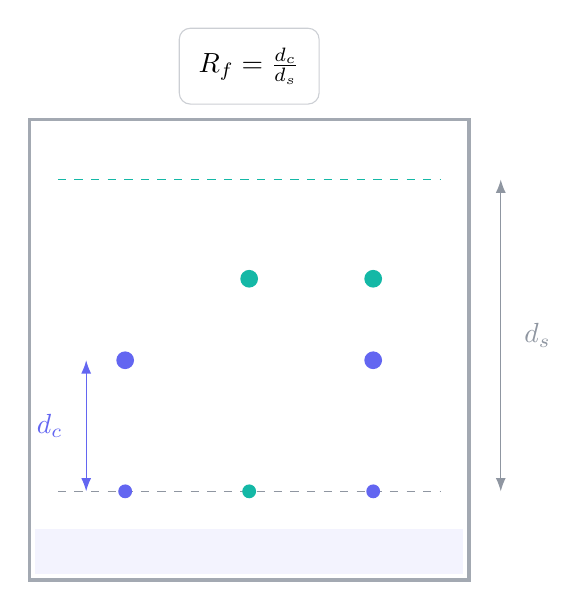
\begin{tikzpicture}[font=\sffamily,>=Latex,x=.9cm,y=.9cm]
  \draw[very thick,ink!45] (0,0) rectangle (6.2,6.5);
  \fill[nebula!8] (.08,.08) rectangle (6.12,.72);
  \draw[dashed,ink!55] (.4,1.25)--(5.8,1.25);
  \draw[dashed,spark] (.4,5.65)--(5.8,5.65);
  \fill[nebula] (1.35,1.25) circle (2.5pt);
  \fill[nebula] (1.35,3.1) circle (3.2pt);
  \fill[spark] (3.1,1.25) circle (2.5pt);
  \fill[spark] (3.1,4.25) circle (3.2pt);
  \fill[nebula] (4.85,1.25) circle (2.5pt);
  \fill[nebula] (4.85,3.1) circle (3.2pt);
  \fill[spark] (4.85,4.25) circle (3.2pt);
  \draw[<->,ink!55] (6.65,1.25)--(6.65,5.65) node[midway,right=5pt] {$d_s$};
  \draw[<->,nebula] (.8,1.25)--(.8,3.1) node[midway,left=5pt] {$d_c$};
  \node[draw=ink!25,rounded corners=4pt,fill=white,inner sep=7pt] at (3.1,7.25)
    {$R_f=\frac{d_c}{d_s}$};
\end{tikzpicture}
\end{document}
